\section{Compiler Implementation}\label{sec:compiler}



%-----------------------------------------------------------------------------
\subsection{Omni XMP Compiler Framework}
%-----------------------------------------------------------------------------

The CAF translator was added into the Omni XMP compiler as shown in Figure~\ref{fig:translator}.
The Omni XMP compiler is a source-to-source translator that converts XMP programs 
into the base language (Fortran or C).  The component `coarray translator' is 
located in front of the XMP translator to solve coarray features previously. 
The output of the decompiler is a standard Fortran/C program that may include 
calls to the XMP runtime library.

The following procedures are generated in advance or in the coarray translator
to initialize static coarray variables prior to the execution of the user program:
\begin{itemize}
\item
The built-in main program calls the translated user program following to 
{\tt xmpf\_traverse\_init}, the entry procedure of initialization routines.
\item
{\tt xmpf\_traverse\_init} is generated by the coarray translator to call 
all initialization routines for all user-defined procedures.
\item
Each initialization routine {\tt xmpf\_init\_{\it foo}} is generated from 
user-defined procedure {\it foo} by the coarray translator. 
It initializes all static coarrays declared in {\it foo}.
\end{itemize}

\begin{figure}[tbh]
 \begin{center}
  % trimはleft bottom right topの順
  %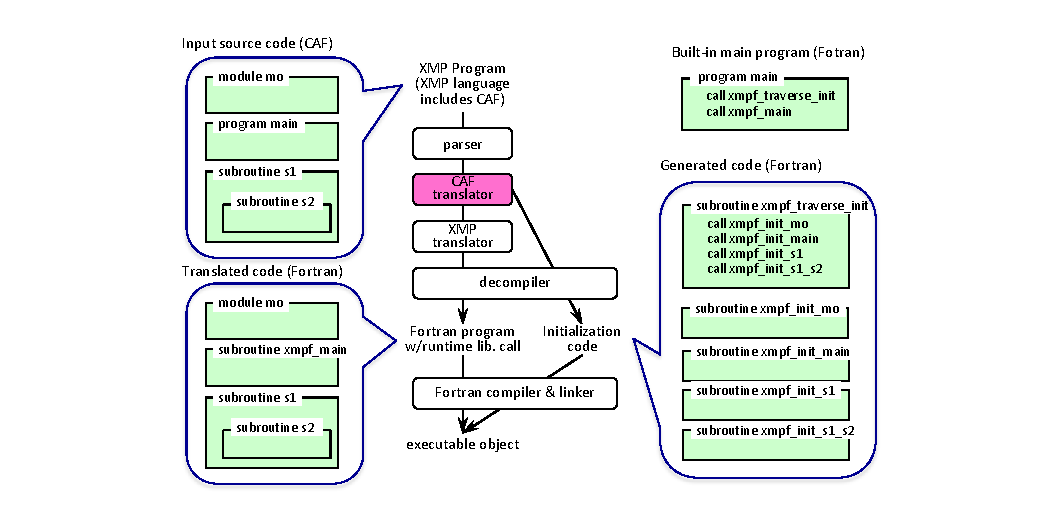
\includegraphics[scale=0.55,trim=6cm 0cm 4cm 6cm,clip]{figs/translator-tmp.pdf}
  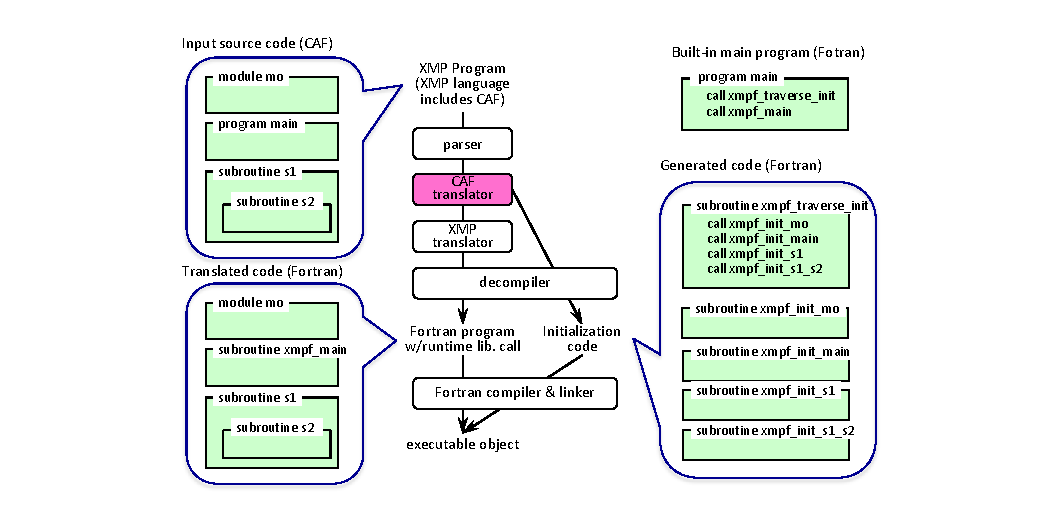
\includegraphics[trim=30mm 0mm 20mm 7mm, scale=1.0]{figs/translator-tmp.pdf}
  \caption{XMP compiler and an example of coarray program compilation}
  \label{fig:translator}
  %-- 修正すべき箇所
  CAF translator $\rightarrow$ coarray translator
 \end{center}
\end{figure}


%-----------------------------------------------------------------------------
\subsection{Allocation of Coarrays}
%-----------------------------------------------------------------------------

To be accessed using the underlying communication library,
the allocated coarray data must be registered to the library.
The registration contains all actions to allow the data to be accessed 
from the other nodes, including pin-down memory, acquirement of the global address,
and sharing information among all nodes.

%===========================================================
\subsubsection{Three methods of memory management}
%===========================================================

The coarray translator and the runtime library implements three methods of
memory management.
\begin{itemize}
\item
The {\bf Runtime Sharing (RS) Method} allocates and registers a large memory 
for all static and dynamic coarrays at the initialization phase.
The registered memory is shared by all static and allocatable coarrays. 

\item
The {\bf Runtime Allocation (RA) Method} allocates and registers a large memory
for all static coarrays at the initialization phase.
And it allocates and registers each allocatable coarray at runtime.

\item
The {\bf Compiler Allocation (CA) Method} allocates all coarray objects by 
the Fortran system (at compile time or at runtime) and the address is 
passed to the runtime library to be registered.
\end{itemize}

For the RS method, the runtime memory has a memory management system for
cutting out and retrieving memory for each allocation and deallocation of 
coarrays.

For the RS and RA methods, 
because the allocated memory address is determined in the runtime library, 
the object code must accept the address allocated 
inside the runtime system as an address of a regal Fortran variable.
To make this connection, it was necessary to use the Cray pointer, which is not 
in the Fortran standard.
In the case of the CA method, the runtime library accepts the address allocated
in the Fortran system, and registers to the communication library.

%
% 3 methodsの比較表を載せるならここか
%


%-----------------------------------------------------------------------------
\subsection{Allocation of Static Coarrays}
%-----------------------------------------------------------------------------

On the {\bf Runtime-library Sharing (RS) method} and 
on the {\bf Runtime-library Allocation (RA) method},
static coarrays are initialized before the execution of the user program,
as follows.
\begin{itemize}
\item
In the first pass, all sizes of static (non-allocatable) coarrays are summed.
The size of each static coarray is evaluated form the declaration 
statement of each coarray. Because the dimensions may have any 
integer constant expression, the coarray translator 
evaluates name of constants, binary and unary operations, and 
basic Fortran intrinsic functions such as min/max and sum.
\item
Then, the total size of static coarrays is allocated and the address
and the size is registered to the underlying communication library.
\item
In the second pass, the addresses of the all coarrays are calculated to share
the registered data.
Due to the language specification, sizes of the same coarray are the same 
among all images (nodes). So the offset from the base address of the registered 
data for each coarray can be the same among all images.
\end{itemize}

On the {\bf Compiler Allocation (CA) method},
the Fortran processor allocates each coarray and then the runtime library
registers the address.
Each static coarray is converted into a common (external) variable to share 
between the user-defined procedure (say {\it foo}) and its initialization
procedure ({\tt xmpf\_init\_{\it foo}}). The data is statically allocated
by the Fortran system similarly to the usual common variable.
the address is registered in the initialization procedure via the runtime
library.


%-----------------------------------------------------------------------------
\subsection{Allocation of Allocatable Coarrays}
%-----------------------------------------------------------------------------

In the RS method, allocatable coarrays are also share the registered memory
described in the previous subsection. The total size of the memory to be registered
should be specified with an environment variable defined by the user.

Figure~\ref{fig:register-RA-CA} illustrates the memory allocation and registration
for allocatable coarrays on the RA and CA methods. 

\begin{figure}[tbh]
 \begin{center}
  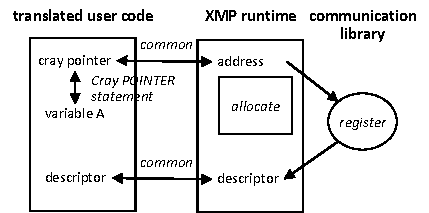
\includegraphics[scale=0.9, trim=0mm 0mm 0mm 0mm, clip]{figs/register-RA-tmp.pdf}\\
The runtime allocates and registers coarrays and passes the address to the user code.
 \end{center}
 \begin{center}
(a) RA method
 \end{center}
 \begin{center}
  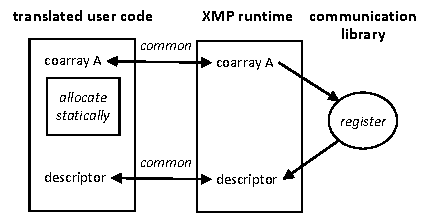
\includegraphics[scale=0.9, trim=0mm 0mm 0mm 0mm, clip]{figs/register-CA-tmp.pdf}\\
The user code allocates coarrays and causes the runtime to register with the address.
 \end{center}
 \begin{center}
(b) CA method
 \end{center}
 \caption{Memory allocation for coarrays in RA and CA methods}
 \label{fig:register-RA-CA}
\end{figure}


These methods are properly used by the underlying communication library.
%
On GASNet, only the RS method is adopted because its allocation function
can be used only once in the program.
%
On MPI-3, the CA method is not suitable because frequent 
allocation and deallocation of coarrays cause expensive creation and freeing 
MPI windows.
%
Over FJ-RDMA, the RS method has no advantage over the other methods.
Since the allocated address is used for registration to FJ-RDMA, 
no advantage was found for managing memory outside of the Fortran system. 
The unusual connection through the Cray pointer causes the degrade of 
the Fortran compiler optimization.


%-----------------------------------------------------------------------------
\subsection{PUT/GET Communication}
%-----------------------------------------------------------------------------

To avoid disturbing the execution on the remote image, PUT and GET communications
are implemented always using Remote Direct Memory Access (RDMA) provided by 
the communication library (except coarrays with pointer/allocatable structure components). 
In contrast, local data access is selective between using Direct Memory Access (DMA) or
using a local buffer. For the buffer scheme, one of four algorithms will be chosen 
depending on three parameters, the size of the local buffer $B$ and the 
local and remote contiguous lengths $N_L$ and $N_R$.
$B$ should be large enough to ignore communication latency overhead and we use
about 400 kilo-bites in default. Unlike the case of MPI message passing,
coarray PUT/GET communication requires only one local buffer for any numbers of
other images.
$N_L$ and $N_R$ can be evaluated at runtime. The Fortran syntax guarantees 
that $N_L$ is a multiple of $N_R$ or $N_R$ is a multiple of $N_L$.
An algorithm to get the contiguous length is shown in the paper~\cite{pgas15}.

\tab{putget} summarizes our algorithm for PUT/GET communication for five cases.
The unit size is the chunk length of the PUT/GET communication.
Case~0 shows the algorithm using RDMA-DMA PUT/GET communication and Cases~1 through~4
shows the algorithms using RDMA and local-buffering. 
Due to its strict condition, the DMA scheme is rarely used.
And it is not always faster than the buffering scheme cases~2 and~3 because of the 
difference of the unit sizes. The merit of cases~2 and~3 is that the unit size 
is extended to a multiple of $N_L$ by gathering number of short contiguous data in the buffer,
or by scattering from the buffer into number of short contiguous data.

\begin{table}[tbh]
 \caption{Summary of the PUT/GET algorithm related to $N_L$, $N_R$ and $B$}
 \label{tab:putget}
 \begin{flushleft}
  \begin{tabular}{|@{~}c@{~}|c||@{~}c@{~}|@{~}c@{~}|}
\hline
scheme &
case &
condition &
unit size \\
\hline
\hline
DMA &
&
Local data is registered. &
$\min(N_L, N_R)$ \\
\hline
buffering &
1 & 
$N_R \leq B,~ N_R \leq N_L$ &
$N_R$ \\
\cline{2-4}
&
2 &
$N_L < N_R \leq B$ &
$N_R$ \\
\cline{2-4}
&
3 &
$N_L < B < N_R$ &
multiple of $N_L$ ($\leq B$) \\
\cline{2-4}
&
4 &
$B < N_R,~ B \leq N_L$ &
$B$ (or less than $B$ at last) \\
\hline
  \end{tabular}
 \end{flushleft}
 \begin{flushleft}
  \begin{tabular}{|@{~}c@{~}|c||@{~~}l@{~~}|@{~~}l@{~~}|}
\hline
scheme &
case &
PUT action for every unit &
GET action for every unit \\
\hline
\hline
DMA &
&
put once &
get once \\
\hline
buffering &
1 &
buffer once and put once &
get once and unbuffer once \\
\cline{2-4}
&
2 &
buffer for each $N_L$, and put once &
get once, and unbuffer for each $N_L$ \\
\cline{2-4}
&
3 &
buffer for each $N_L$, and put once &
get once, and unbuffer for each $N_L$ \\
\cline{2-4}
&
4 &
buffer once and put once &
get once and unbuffer once \\
\hline
  \end{tabular}
 \end{flushleft}
\end{table}



%-----------------------------------------------------------------------------
\subsection{Non-blocking one-sided communication}
%-----------------------------------------------------------------------------

Get通信をできる限りnon-blockingとし、そして、その完了待ちを可能なら次のimage control statementまで遅延したい。
\fig{block-ex}に示したような、同じsegment内で同じリモートデータへ書いて読むような
ケースは大変まれで、殆どの場合には次のimage control statementまで遅延できる。
添字式やイメージ番号が定数でないことが多いので、コンパイル時の判定では遅い方に倒れてしまう。
まれなケースを除外するための実行時判定が望まれる。

正確な実行時判定を行うためには、現在non-blocking PUT通信中のcoarrayのアドレスのrangeと相手のimage番号を
ハッシュテーブルに記憶し、GET通信を行う前にそのrangeとimage番号に重なりがないことをチェックし、
重なりがあったらそこでPUT通信を完了させる、という方法が考えられる。
しかしこれでは、重なりが無い通常のケースでも重なりのチェックのコストが大きい。
コンパイラでの解析と動的なチェックを併用する、正確さが劣ってもより高速な方法が望ましい。

現在の実装では、実行時の環境変数によってblockingとnon-blocking通信を選択する。
以下の条件に該当する場合には、低速となるblockingを選択しなければならない。
 明示的な同期なしで、リモートのcoarray変数に対して定義後の参照がある。



